\section{Experiments}
\label{sec:experiments}

\subsection{Simulation Study}\label{sec:sim1}

\begin{figure}[ht]
    \centering
    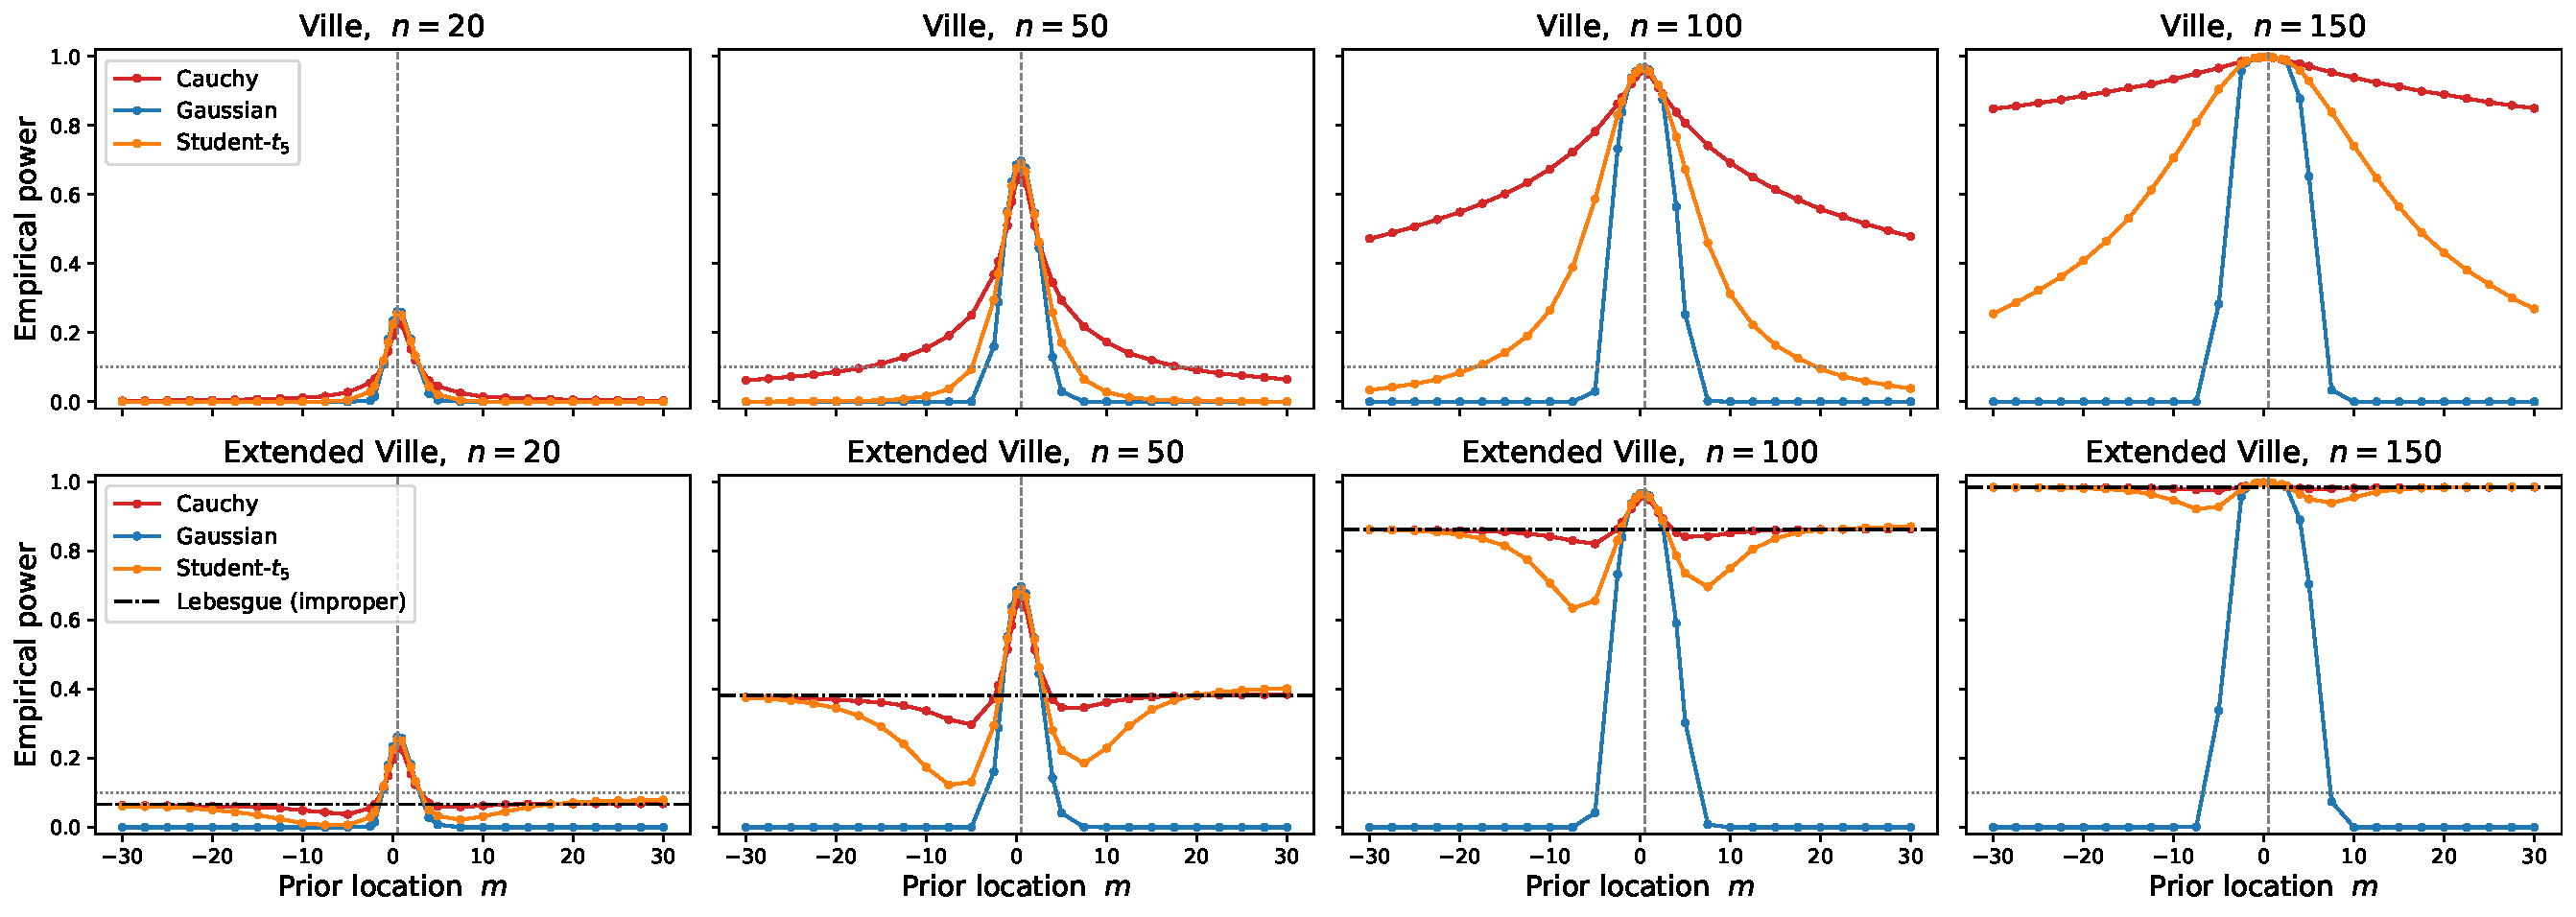
\includegraphics[width=\linewidth, height=0.4\linewidth]{JRSSB/images/power_vs_m_priors.pdf}
    \caption{Empirical power of the Ville (top row) and extended-Ville (bottom row)
    procedures against the prior location \(m\), for \(H_0:\theta=0\) against
    \(H_1:\theta\neq0\) with \(\theta^\star=0.5\) and \(n\in\{20,50,100,150\}\);
    \(B=10{,}000\) data replicates and \(B_{\mathrm{cal}}=100{,}000\) calibration
    replicates. The dashed vertical line marks the well-specified location
    \(m=\theta^\star\), the dotted horizontal line the level \(\alpha=0.1\), and the
    dash-dotted black line in the bottom row the non-informative Lebesgue baseline.}
    \label{fig:power_vs_m_priors}
\end{figure}

We illustrate the theory through a simulation study and visualise the empirical power vs prior location. Throughout we set \(\sigma=1\), so the data generated from $\mathcal{N}(0.5, 1)$ coincides with the standardised effect size \(\theta^\star = 0.5\). Let us now consider the anytime-valid test of \(H_0:\theta=0\) against \(H_1:\theta\neq0\) at fixed sample size \(n\) with level \(\alpha = 0.1\), and consider \(n\in\{20,50,100,150\}\). For each prior \(\pi\) and each location \(m\) on the grid \(\mathcal M\) on \([-30, 30]\), we draw \(B=10{,}000\) datasets
\(Y_{1:n}^{(b)}\stackrel{\mathrm{iid}}{\sim}\mathcal N(\theta^\star,1)\)
and report the empirical Ville and extended-Ville rejection rates,
\(\widehat{\mathrm{pow}}^{V}_{n,\alpha}(m)\) and
\(\widehat{\mathrm{pow}}^{eV}_{n,\alpha}(m)\), defined as the fraction
of replicates for which the corresponding \(p\)-variable falls at or
below \(\alpha\).

\begin{figure}
    \centering
    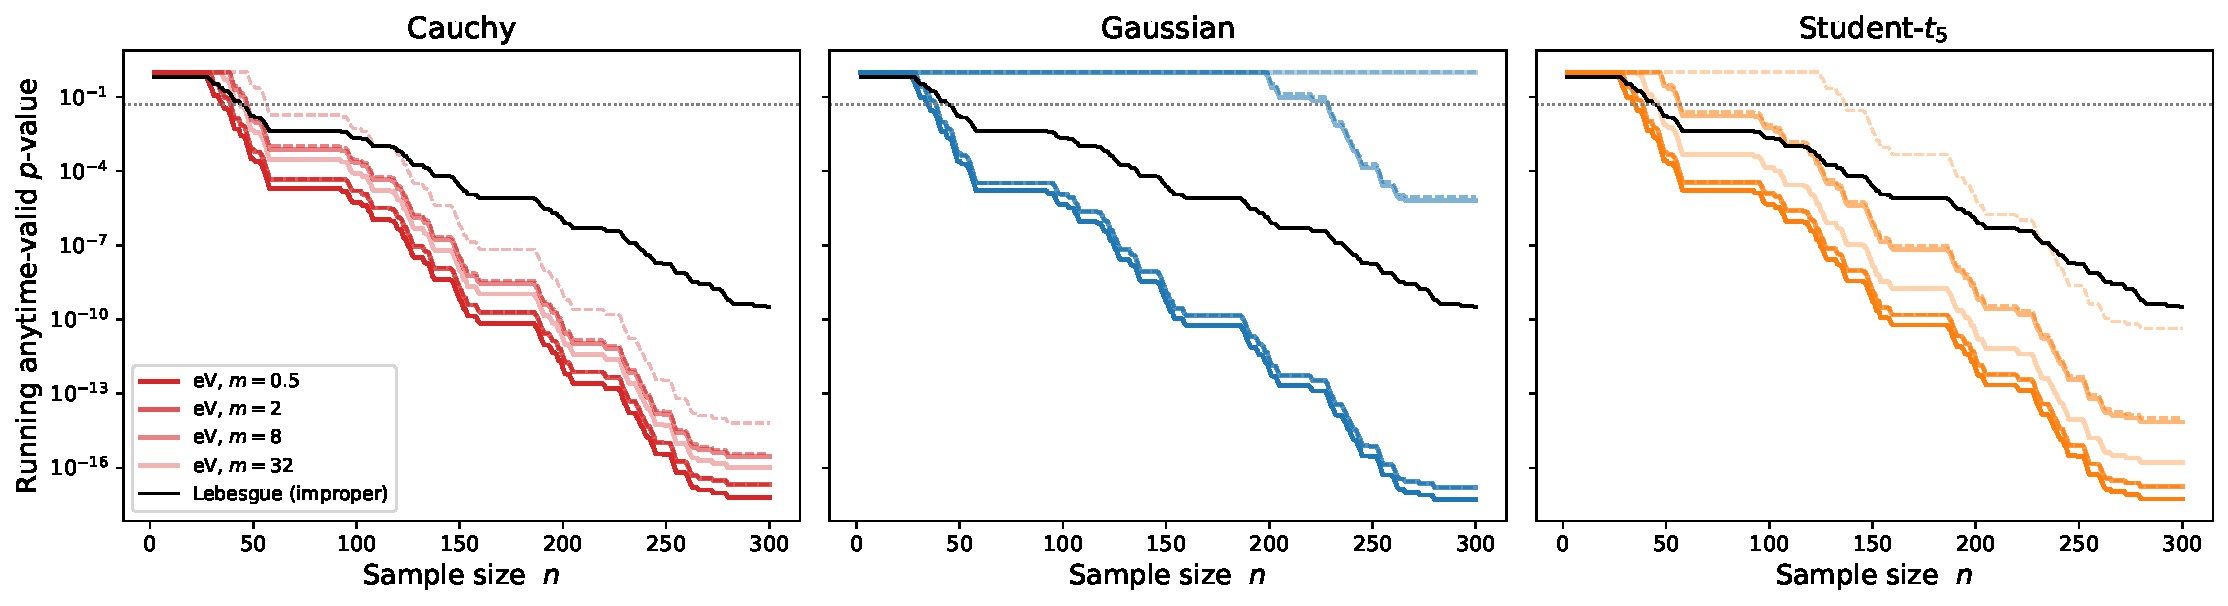
\includegraphics[width=\linewidth]{JRSSB/images/pvalue_vs_n_simulated.pdf}
    \caption{Running anytime-valid \(p\)-values against sample size \(n\), on a
    logarithmic vertical scale, for the Cauchy, Gaussian and Student-\(t_5\) priors
    at prior locations \(m\in\{0.5,2,8,32\}\); one stream with \(\theta^\star=0.5\),
    \(\alpha=0.05\). Solid curves give the extended-Ville and dashed curves the Ville
    \(p\)-process, lighter shading corresponding to larger \(m\); the black curve is
    the non-informative Lebesgue baseline and the dotted horizontal line the level
    \(\alpha\). Both processes are evaluated at the running maximum of the wealth
    process and are therefore non-increasing in \(n\). 
    }
    \label{fig:pvalue_vs_n_simulated}
\end{figure}


We compare the proper priors Cauchy (with the Rouder-JZS default scale $\frac{1}{\sqrt{2}} \approx 0.707$), Gaussian (with $\sigma = 1$) and Student-\(t\) (with degrees of freedom $5$ and scale $=1$); the improper Lebesgue prior of Section~\ref{subsec:improper-prior} serves as a non-informative baseline in the extended-Ville. The marginal likelihoods \(M_n^{\Pi_m}\) admit no closed form for these priors and are computed by adaptive Gauss-Kronrod quadrature in \(\theta\) \citep{piessens2012quadpack}, while the calibration functions
\(g_0^{(m)}\) are obtained by Monte Carlo under \(\Prob_0\) with
\(B_{\mathrm{cal}}=100{,}000\) replicates. Note that the law of \(M_2^{\Pi_m}(Y_{1:2})\) under \(\Prob_0\) depends on \(m\), so the calibration must be recomputed across the grid; however a single \(\Prob_0\)-sample of pairs \((Y_1^{(j)},Y_2^{(j)})\) suffices for the entire grid, since \(M_2^{\Pi_m}(Y_1^{(j)},Y_2^{(j)})\) can be evaluated for every \(m\in\mathcal M\) on the same Monte Carlo draws. The Lebesgue baseline uses the closed-form derived in Proposition~\ref{thm:Mn-Leb}, so it has no Monte Carlo error. Figure~\ref{fig:power_vs_m_priors} shows that both the Ville and the extended-Ville procedure attain their maximum power near the true effect \(\theta^\star=0.5\) and gradually decreases when the prior-data conflict increases. The Ville eventually drops to $0$ while the extended Ville reverts back to the Lebesgue baseline, making it robust against the prior-data conflict. Figure \ref{fig:pvalue_vs_n_simulated} shows anytime valid $p$-values for different priors with varying mean parameter. The Ville is getting worse at rejection compared to the Extended Ville as the prior-data conflict grows.



\subsection{Experiment on Real-Data}
In machine learning, if we train the same architecture multiple times with different random seeds, we get different held-out accuracy. This matters because each observation costs a full training run, which for large models could be days of GPU time. A practitioner who wishes to certify that a training pipeline meets a stated accuracy specification must therefore average over training runs, and the
natural question is how many runs are needed. Since every observation costs a full training run, a procedure that stops as soon as the evidence permits is worth more here than in the settings where observations are given in advance.

The data-generating mechanism is as follows: we use Fashion-MNIST \citep{Xiao2017}, a benchmark of $70{,}000$ grayscale images of size $28\times28$ across ten clothing categories, introduced as a more demanding replacement for MNIST. From it we draw a fixed training pool of $8{,}000$ images and a disjoint evaluation set of $3{,}000$ images, both held constant throughout. We then train $N=1{,}200$ networks independently, so the $Y_i$ are i.i.d. conditional on that evaluation set. Each is a single-hidden-layer multilayer perceptron with $32$ rectified linear units, hence $25{,}450$ trainable parameters, optimised for $100$ epochs by Adam with an $\ell_2$ penalty of $10^{-4}$ on a subsample of $400$ images drawn without replacement from the pool. Network $i$ thus differs from network $j$ in its weight initialisation, in the ordering of its minibatches, and in which subsample of the pool it sees; these are the three sources of variability a practitioner faces on retraining, and the substantial over-parametrisation relative to the $400$ training images is what makes that variability non-negligible. Writing $A_i$ for the accuracy of network $i$ on the fixed evaluation set and $b$ for a benchmark accuracy fixed in advance, the observation stream is $Y_i = A_i - b$, $i=1,\ldots,N$, and we test $H_0:\theta^\star=0$ against a two-sided alternative at level $\alpha=0.05$. The benchmark $b$ is fixed before the sequential test begins and is chosen so that the non-informative Lebesgue procedure crosses $\alpha$ at roughly a quarter of the stream; this is a legibility requirement on the comparison, in the same spirit as choosing an effect size at which to power a study, and no quantity computed from the sequential test enters the choice.

We compare three proper priors, each at its conventional default scale: the Cauchy at the Rouder--JZS scale $1/\sqrt2$, the Student-$t_5$ at unit scale, and the Gaussian with $\sigma=1$; the improper Lebesgue prior of Section~\ref{subsec:improper-prior} serves as the non-informative baseline. Each is swept over the locations $m\in\{0,1,2,4,8,16,32,64\} \cup \{\widehat\theta_N\}$, measured in standardised-effect units, so that increasing $m$ increases prior--data conflict directly while holding the prior shape and width fixed. For each prior and each location we record, under both the Ville and the extended-Ville constructions, the first index $n$ at which the running $p$-variable falls to $\alpha$ or below, that is, the number of networks that must be trained before the specification can be rejected. The mixture statistics $M_n^{\Pi_m}$ admit no closed form for these priors and are computed by adaptive Gauss--Kronrod quadrature in $\theta$ \citep{piessens2012quadpack}, while the calibration functions $g^{(m)}$ are obtained by Monte Carlo under $\Prob_0$ with $B_{\mathrm{cal}}=100{,}000$ replicates; the Lebesgue baseline uses the closed form of Proposition~\ref{thm:Mn-Leb} and so incurs no Monte Carlo error. Both $p$-processes are evaluated at the running maximum of the wealth process, so that each is non-increasing in $n$.


\begin{figure}
    \centering
    \includegraphics[width=0.8\linewidth]{images/nn_first_rejection_vs_m.pdf}
    \caption{Number of networks that must be trained before the specification
    $H_0:\theta^\star=0$ is rejected at level $\alpha=0.05$, against the prior
    location $m$, for the Cauchy ($r=1/\sqrt2$), Student-$t_5$ ($r=1$) and
    Gaussian ($\sigma=1$) priors. Open circles denote the Ville construction
    and filled squares the extended Ville construction; the dotted horizontal
    line marks the non-informative Lebesgue baseline and the dashed vertical
    line the well-specified location $m=\widehat\theta_N$. Points in the
    shaded band at the top failed to reject within the $N=1{,}200$ available
    runs. The horizontal axis is on a symmetric-log scale.}
    \label{fig:nn-first-rejection}
\end{figure}

\begin{figure}
    \centering
    \includegraphics[width=\linewidth]{images/nn_pvalue_trajectories.pdf}
    \caption{Running anytime-valid $p$-values against the number of networks
    trained, for six prior locations $m$ under each of the three prior
    families. Solid curves give the extended-Ville $p$-process and dashed
    curves the Ville $p$-process; the grey curve is the non-informative
    Lebesgue baseline and the dotted horizontal line the level $\alpha=0.05$.
    Lighter shading corresponds to larger $m$, that is, to greater
    prior--data conflict. Both $p$-processes are evaluated at the running
    maximum of the wealth process and are therefore non-increasing in $n$.}
    \label{fig:nn-trajectories}
\end{figure}

Figure~\ref{fig:nn-first-rejection} show the number of networks trained before rejection against the prior mean (in $\log_2$ scale) and Figure~\ref{fig:nn-trajectories} plots the running anytime-valid $p$-value against the number of networks trained. The Lebesgue procedure rejects after $165$ runs; at locations at or near the truth all three families reject after roughly $140$. As $m$ increases the families separate. The Gaussian prior requires $585$ runs at $m=8$ and fails to reject at all for $m\geq16$, exhausting the budget of $1{,}200$ runs. The Cauchy and Student-$t_5$ priors rise briefly over $m\in[4,16]$ and then
return to the Lebesgue baseline at $m=32$ and $m=64$, so that a polynomial-tail prior asserting an effect two orders of magnitude beyond the truth costs nothing relative to using no prior information; this is the recovery of Theorem~\ref{thm:recovery}, against the failure of the Gaussian. Across every prior and every location the extended-Ville first-rejection time is at or before its Ville counterpart, and the gap is largest under severe conflict: at $m=32$ with the Student-$t_5$ prior, extended Ville rejects after $165$ runs against $535$ for Ville, a saving of $370$ training runs.


% \begin{figure}[h]
%     \centering
%     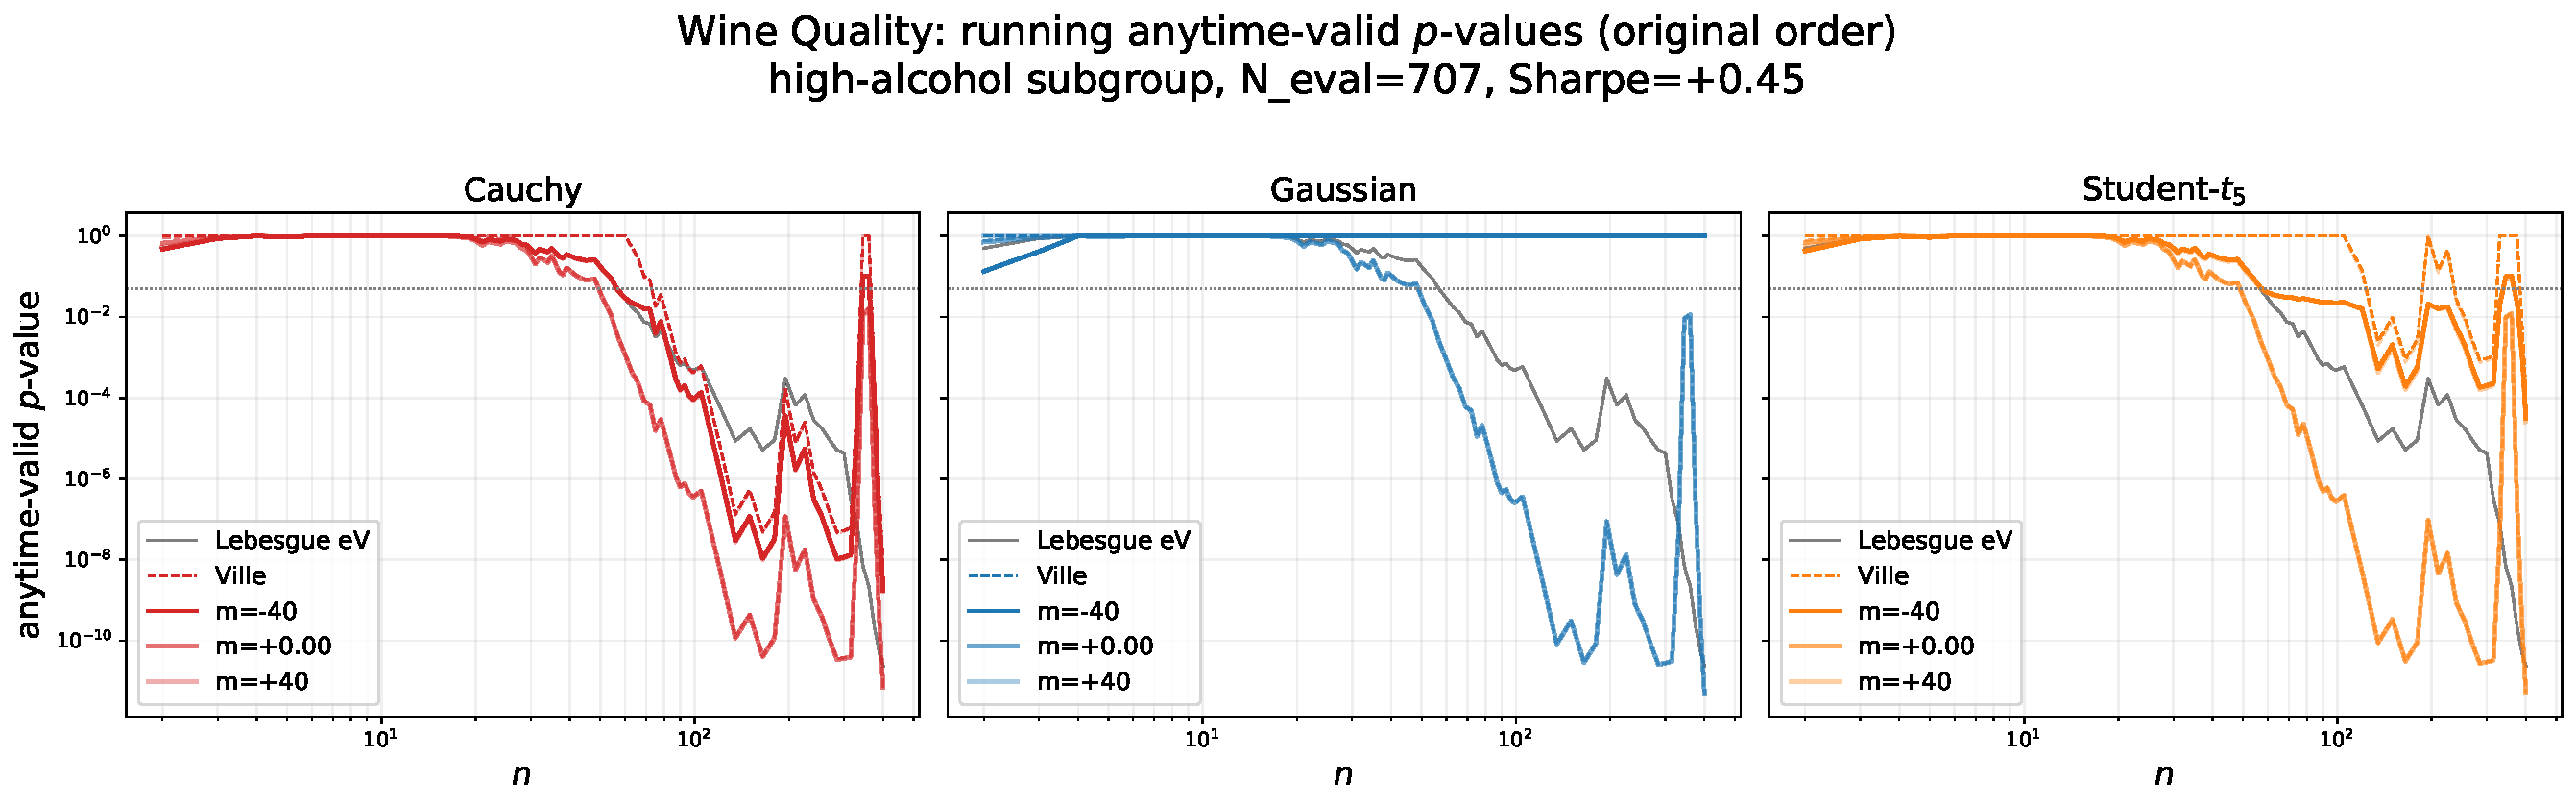
\includegraphics[width=\linewidth]{images/wine_pvalue_trajectory.pdf}
%     \caption{Anytime-valid $p$-value trajectories for the Wine Quality dataset under five prior families. Solid lines represent the Extended Ville procedure, dashed lines the Ville procedure, and the thin black line the Lebesgue e-value baseline. Darker curves correspond to prior locations closer to the empirical data mean.}
%     \label{fig:wine_pval_trajectory}
% \end{figure}

% We now turn from simulated data to a real dataset, where the effect is fixed by the data. We use the red-wine subset of the wine-quality data of \citet{Cortez2009}, which records a sensory quality score, on an integer scale, for each of $1{,}599$ wines together with their physicochemical properties. To obtain a one-sample problem with a genuine effect, we split the wines by alcohol content, which is among the strongest correlates of quality, and ask whether the above-median-alcohol wines differ in quality from the sample as a whole. Let $Y_i$ denote the quality score of high-alcohol wine $i$, centred at the overall mean, and let $\theta^\star = \mathbb{E}[Y_i]/\sqrt{\operatorname{Var}(Y_i)}$ be its standardised effect. We test $H_0:\theta^\star=0$ against a two-sided alternative, the scale-invariant problem of Section~\ref{subsec:improper-prior} with unknown variance. 

% \begin{figure}[h]
%     \centering
%     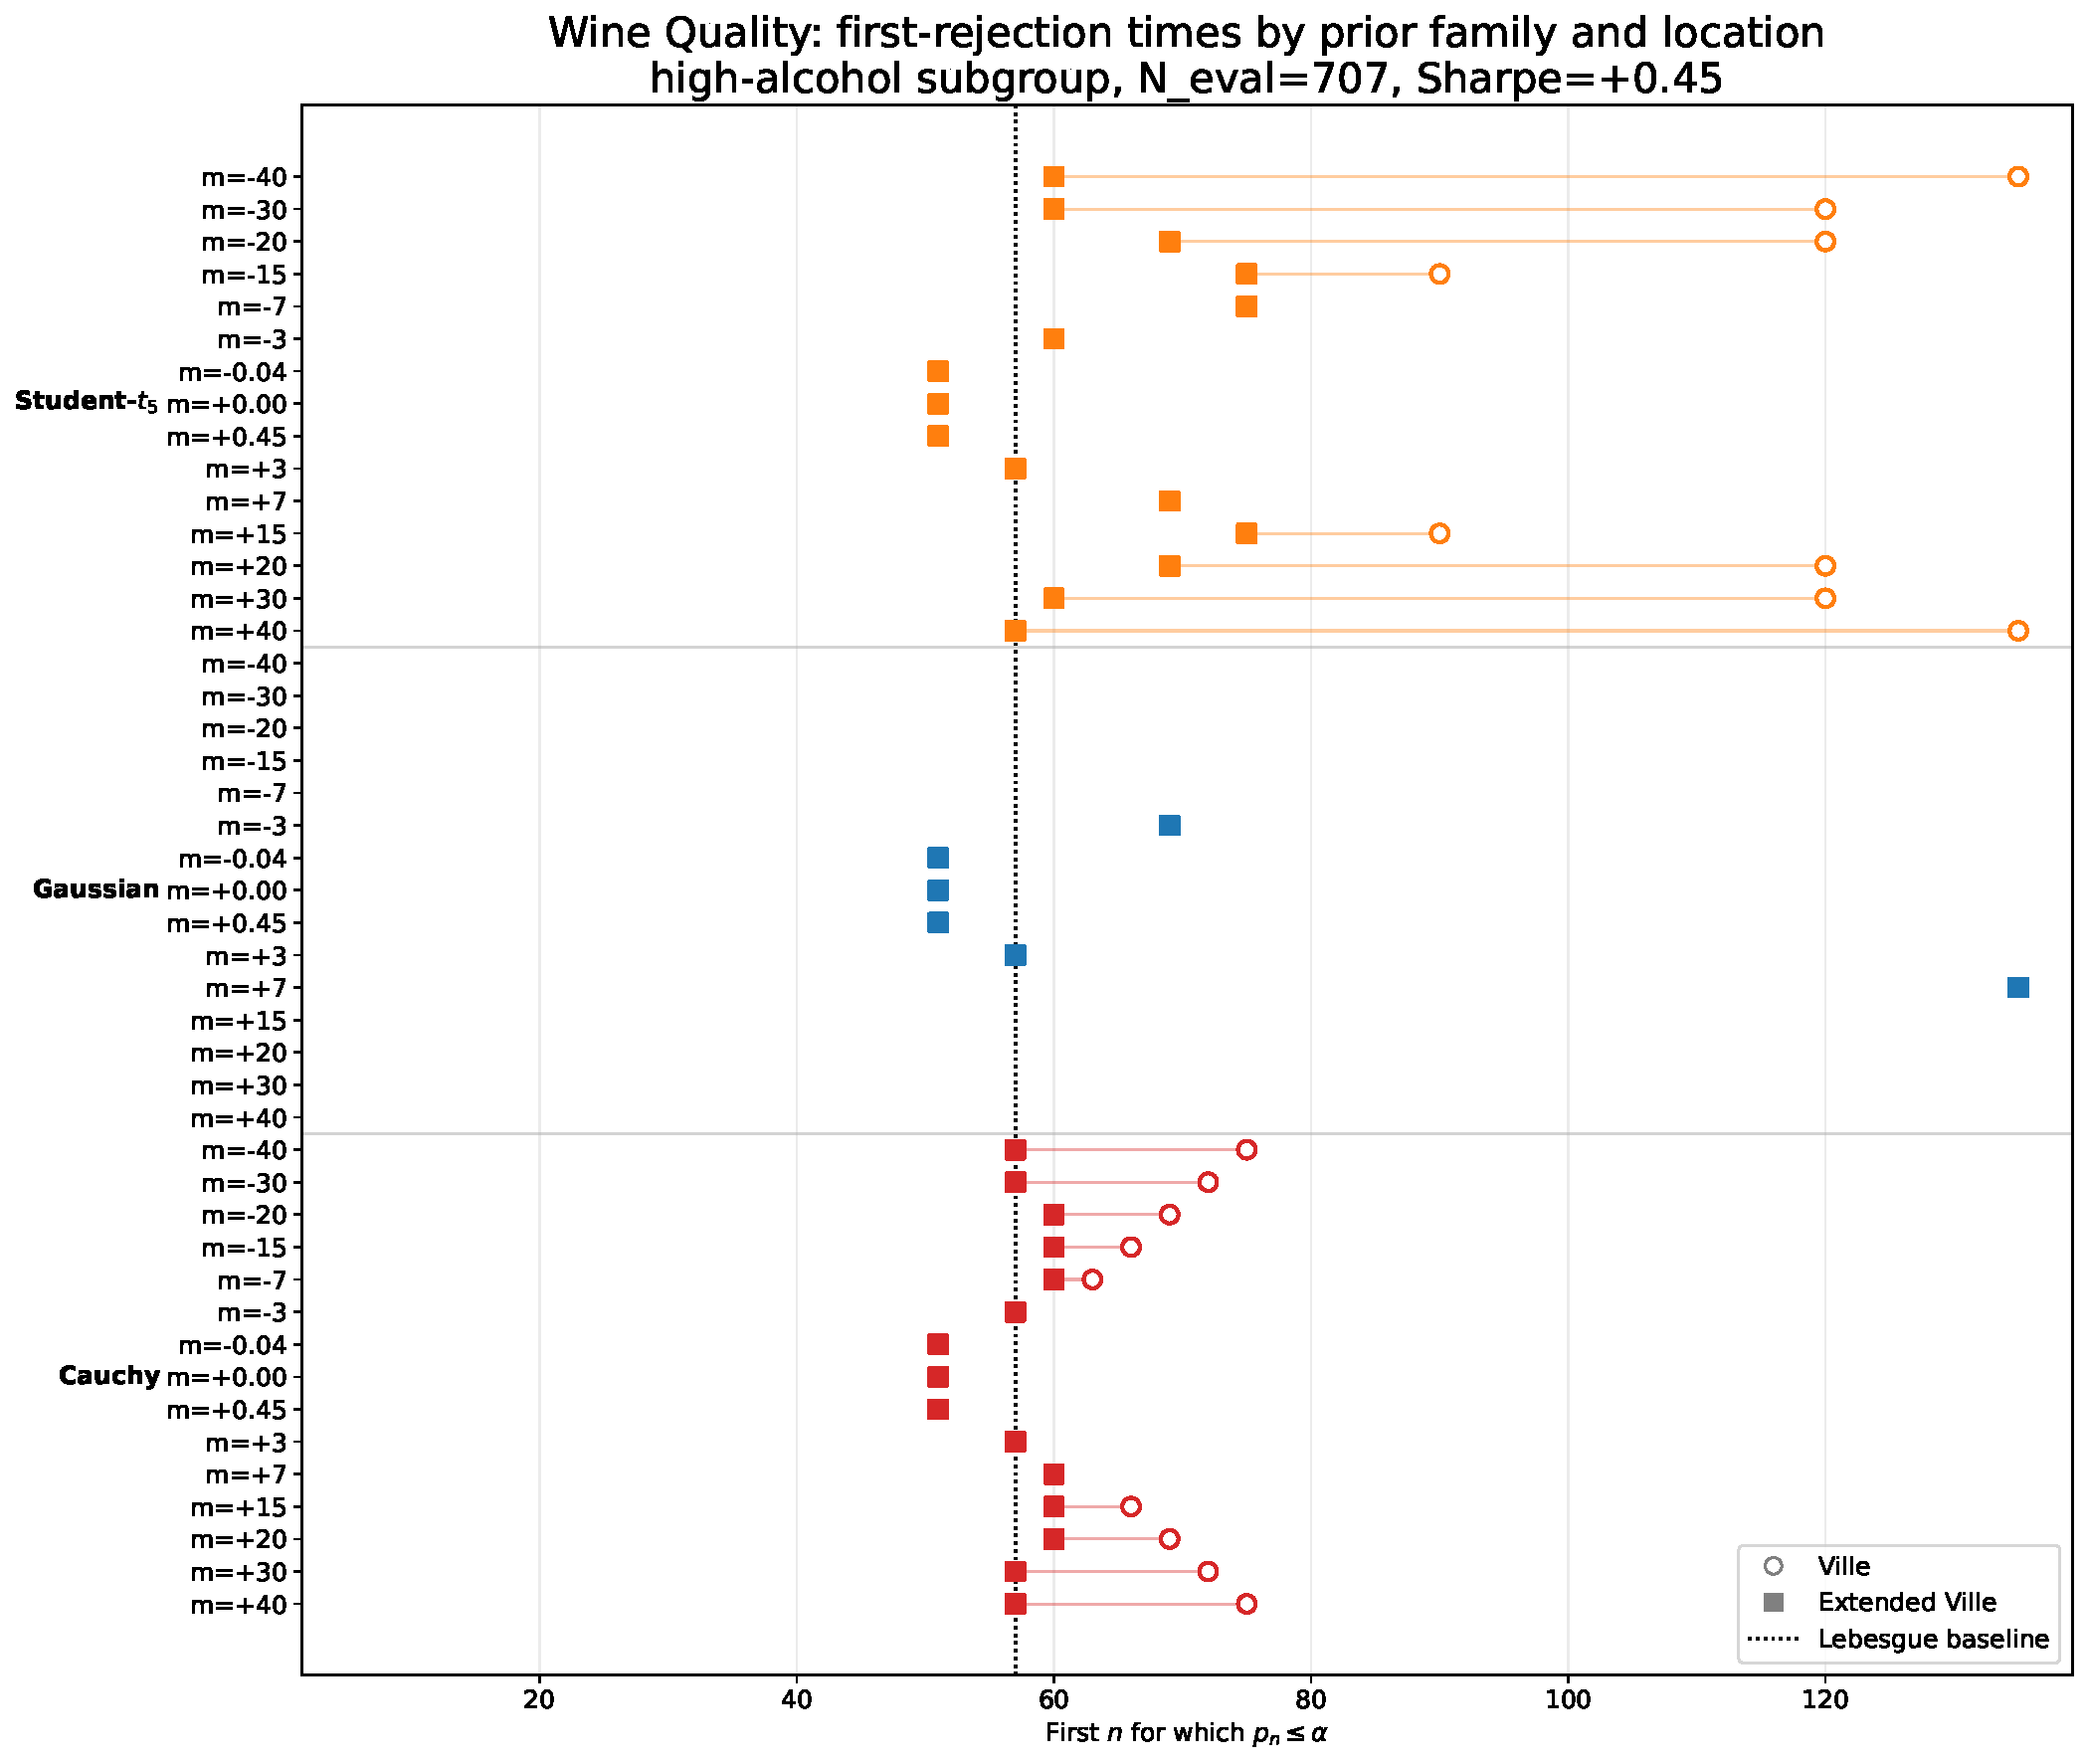
\includegraphics[width=\linewidth]{images/wine_first_rejection.pdf}
%     \caption{First rejection time ($n$) at which $p_n \leq \alpha$ for the Wine Quality dataset, evaluated across multiple prior families and location parameters. Results are shown for the Ville (circles) and Extended Ville (squares) procedures, with the Lebesgue baseline indicated by the dotted vertical line ($n=57$).}
%     \label{fig:wine_first_rej}
% \end{figure}

% Rather than fix the prior location in advance, we estimate it from a pilot sample. We hold out the first $N_{\mathrm{cal}}=50$ observations out of the $757$ of the subgroup as a pilot set $\mathcal C$ and take the prior location to be its sample Sharpe ratio, $\widehat m_{\mathrm{EB}}=\bar Y_{\mathcal C}/S_{\mathcal C}$. The remaining $N_{\mathrm{eval}}=707$ observations form the sequence on which the anytime-valid procedures are run with the standardised effect is $\widehat\theta_N\approx 0.45$. We take $\alpha=0.05$ throughout. We use the same priors and grid of locations $m$ as in Section~\ref{sec:sim1}, now ranging from the pilot estimate $\widehat m_{\mathrm{EB}}$ out to severe prior-data conflict at $|m|=40$, with the improper Lebesgue prior of Section~\ref{subsec:improper-prior} as the non-informative baseline.

% Figures~\ref{fig:wine_pval_trajectory} and~\ref{fig:wine_first_rej} exhibit the same qualitative behaviour as in the simulations. The Extended Ville procedure is uniformly at least as efficient as the Ville procedure, with the advantage becoming most pronounced when the prior location is substantially misspecified.



